\documentclass[1p]{elsarticle_modified}
%\bibliographystyle{elsarticle-num}

%\usepackage[colorlinks]{hyperref}
%\usepackage{abbrmath_seonhwa} %\Abb, \Ascr, \Acal ,\Abf, \Afrak
\usepackage{amsfonts}
\usepackage{amssymb}
\usepackage{amsmath}
\usepackage{amsthm}
\usepackage{scalefnt}
\usepackage{amsbsy}
\usepackage{kotex}
\usepackage{caption}
\usepackage{subfig}
\usepackage{color}
\usepackage{graphicx}
\usepackage{xcolor} %% white, black, red, green, blue, cyan, magenta, yellow
\usepackage{float}
\usepackage{setspace}
\usepackage{hyperref}

\usepackage{tikz}
\usetikzlibrary{arrows}

\usepackage{multirow}
\usepackage{array} % fixed length table
\usepackage{hhline}

%%%%%%%%%%%%%%%%%%%%%
\makeatletter
\renewcommand*\env@matrix[1][\arraystretch]{%
	\edef\arraystretch{#1}%
	\hskip -\arraycolsep
	\let\@ifnextchar\new@ifnextchar
	\array{*\c@MaxMatrixCols c}}
\makeatother %https://tex.stackexchange.com/questions/14071/how-can-i-increase-the-line-spacing-in-a-matrix
%%%%%%%%%%%%%%%

\usepackage[normalem]{ulem}

\newcommand{\msout}[1]{\ifmmode\text{\sout{\ensuremath{#1}}}\else\sout{#1}\fi}
%SOURCE: \msout is \stkout macro in https://tex.stackexchange.com/questions/20609/strikeout-in-math-mode

\newcommand{\cancel}[1]{
	\ifmmode
	{\color{red}\msout{#1}}
	\else
	{\color{red}\sout{#1}}
	\fi
}

\newcommand{\add}[1]{
	{\color{blue}\uwave{#1}}
}

\newcommand{\replace}[2]{
	\ifmmode
	{\color{red}\msout{#1}}{\color{blue}\uwave{#2}}
	\else
	{\color{red}\sout{#1}}{\color{blue}\uwave{#2}}
	\fi
}

\newcommand{\Sol}{\mathcal{S}} %segment
\newcommand{\D}{D} %diagram
\newcommand{\A}{\mathcal{A}} %arc


%%%%%%%%%%%%%%%%%%%%%%%%%%%%%5 test

\def\sl{\operatorname{\textup{SL}}(2,\Cbb)}
\def\psl{\operatorname{\textup{PSL}}(2,\Cbb)}
\def\quan{\mkern 1mu \triangleright \mkern 1mu}

\theoremstyle{definition}
\newtheorem{thm}{Theorem}[section]
\newtheorem{prop}[thm]{Proposition}
\newtheorem{lem}[thm]{Lemma}
\newtheorem{ques}[thm]{Question}
\newtheorem{cor}[thm]{Corollary}
\newtheorem{defn}[thm]{Definition}
\newtheorem{exam}[thm]{Example}
\newtheorem{rmk}[thm]{Remark}
\newtheorem{alg}[thm]{Algorithm}

\newcommand{\I}{\sqrt{-1}}
\begin{document}

%\begin{frontmatter}
%
%\title{Boundary parabolic representations of knots up to 8 crossings}
%
%%% Group authors per affiliation:
%\author{Yunhi Cho} 
%\address{Department of Mathematics, University of Seoul, Seoul, Korea}
%\ead{yhcho@uos.ac.kr}
%
%
%\author{Seonhwa Kim} %\fnref{s_kim}}
%\address{Center for Geometry and Physics, Institute for Basic Science, Pohang, 37673, Korea}
%\ead{ryeona17@ibs.re.kr}
%
%\author{Hyuk Kim}
%\address{Department of Mathematical Sciences, Seoul National University, Seoul 08826, Korea}
%\ead{hyukkim@snu.ac.kr}
%
%\author{Seokbeom Yoon}
%\address{Department of Mathematical Sciences, Seoul National University, Seoul, 08826,  Korea}
%\ead{sbyoon15@snu.ac.kr}
%
%\begin{abstract}
%We find all boundary parabolic representation of knots up to 8 crossings.
%
%\end{abstract}
%\begin{keyword}
%    \MSC[2010] 57M25 
%\end{keyword}
%
%\end{frontmatter}

%\linenumbers
%\tableofcontents
%
\newcommand\colored[1]{\textcolor{white}{\rule[-0.35ex]{0.8em}{1.4ex}}\kern-0.8em\color{red} #1}%
%\newcommand\colored[1]{\textcolor{white}{ #1}\kern-2.17ex	\textcolor{white}{ #1}\kern-1.81ex	\textcolor{white}{ #1}\kern-2.15ex\color{red}#1	}

{\Large $\underline{12a_{0172}~(K12a_{0172})}$}

\setlength{\tabcolsep}{10pt}
\renewcommand{\arraystretch}{1.6}
\vspace{1cm}\begin{tabular}{m{100pt}>{\centering\arraybackslash}m{274pt}}
\multirow{5}{120pt}{
	\centering
	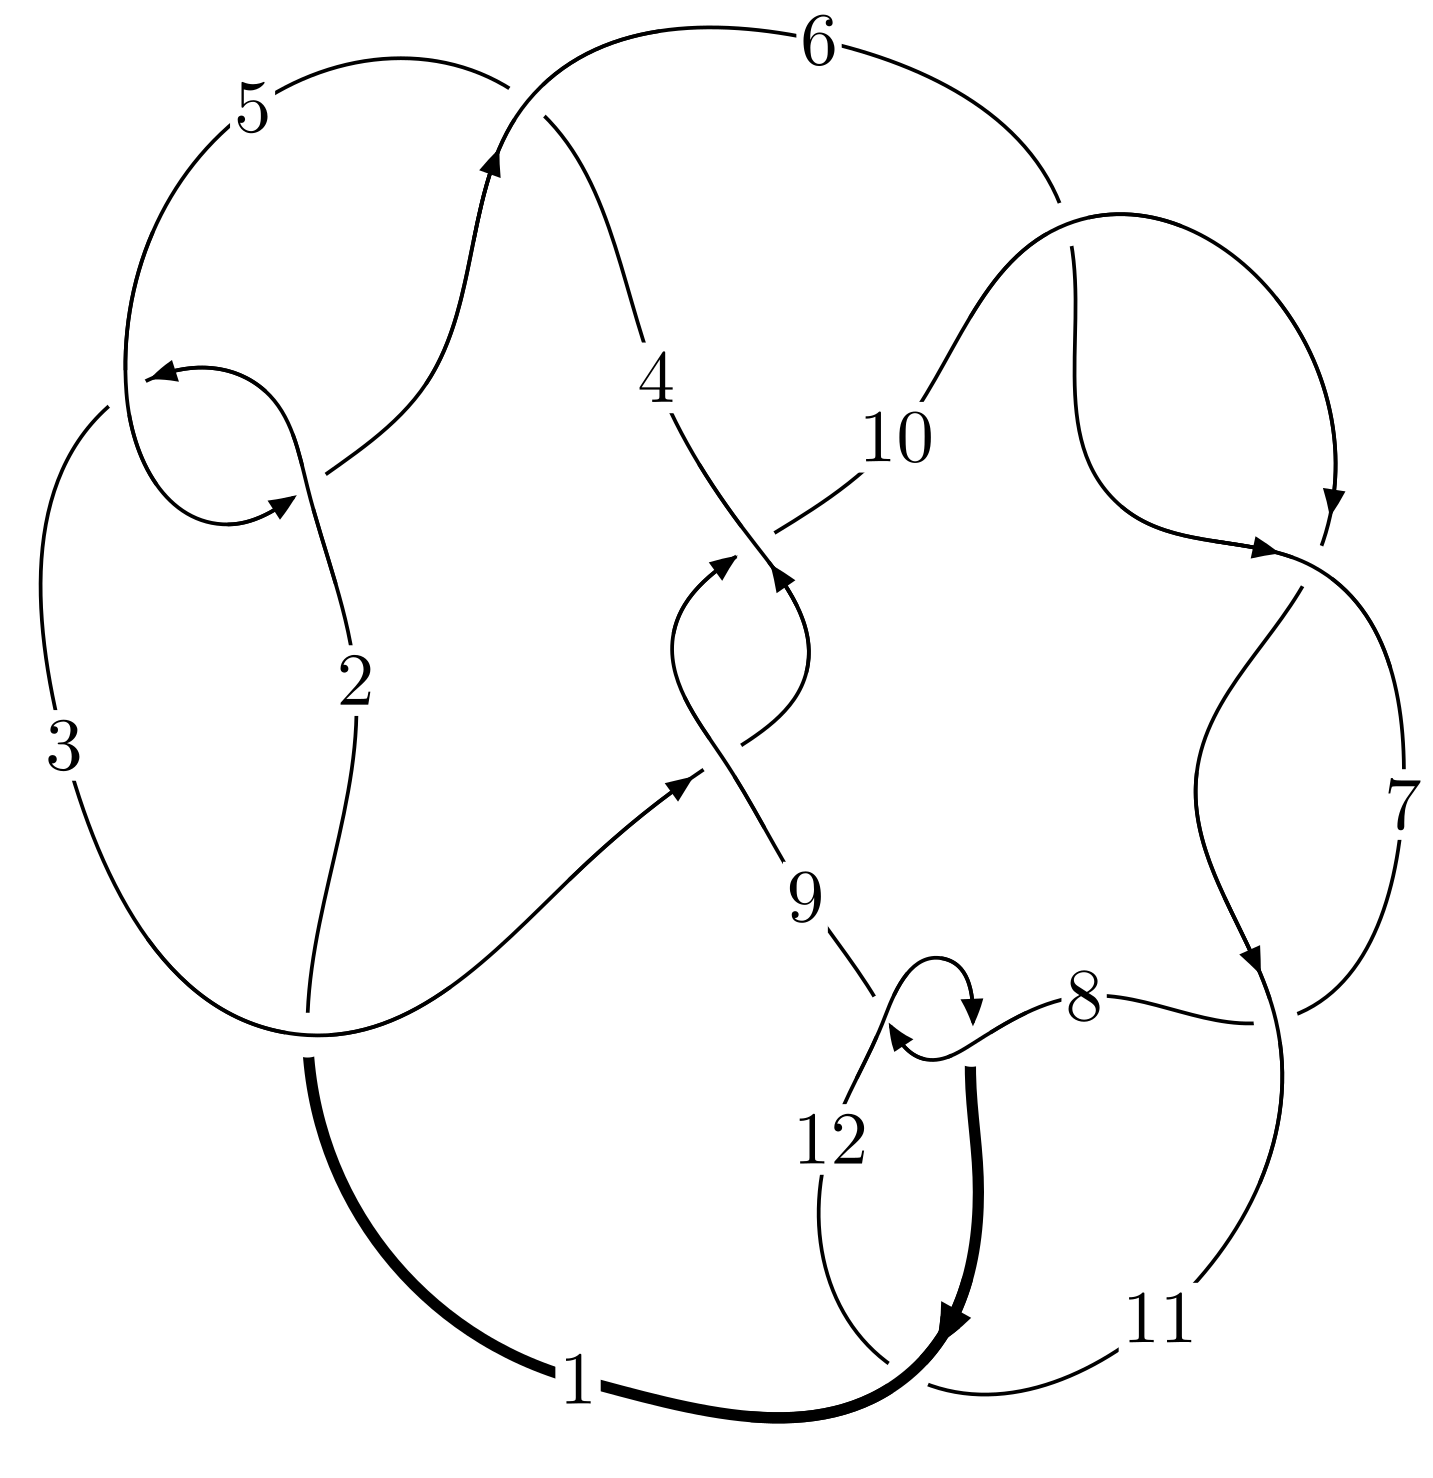
\includegraphics[width=112pt]{../../../GIT/diagram.site/Diagrams/png/973_12a_0172.png}\\
\ \ \ A knot diagram\footnotemark}&
\allowdisplaybreaks
\textbf{Linearized knot diagam} \\
\cline{2-2}
 &
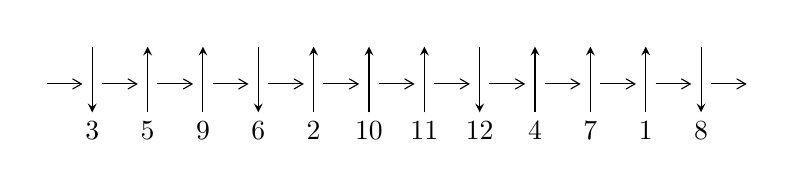
\begin{tikzpicture}[x=20pt, y=17pt]
	% nodes
	\node (C0) at (0, 0) {};
	\node (C1) at (1, 0) {};
	\node (C1U) at (1, +1) {};
	\node (C1D) at (1, -1) {3};

	\node (C2) at (2, 0) {};
	\node (C2U) at (2, +1) {};
	\node (C2D) at (2, -1) {5};

	\node (C3) at (3, 0) {};
	\node (C3U) at (3, +1) {};
	\node (C3D) at (3, -1) {9};

	\node (C4) at (4, 0) {};
	\node (C4U) at (4, +1) {};
	\node (C4D) at (4, -1) {6};

	\node (C5) at (5, 0) {};
	\node (C5U) at (5, +1) {};
	\node (C5D) at (5, -1) {2};

	\node (C6) at (6, 0) {};
	\node (C6U) at (6, +1) {};
	\node (C6D) at (6, -1) {10};

	\node (C7) at (7, 0) {};
	\node (C7U) at (7, +1) {};
	\node (C7D) at (7, -1) {11};

	\node (C8) at (8, 0) {};
	\node (C8U) at (8, +1) {};
	\node (C8D) at (8, -1) {12};

	\node (C9) at (9, 0) {};
	\node (C9U) at (9, +1) {};
	\node (C9D) at (9, -1) {4};

	\node (C10) at (10, 0) {};
	\node (C10U) at (10, +1) {};
	\node (C10D) at (10, -1) {7};

	\node (C11) at (11, 0) {};
	\node (C11U) at (11, +1) {};
	\node (C11D) at (11, -1) {1};

	\node (C12) at (12, 0) {};
	\node (C12U) at (12, +1) {};
	\node (C12D) at (12, -1) {8};
	\node (C13) at (13, 0) {};

	% arrows
	\draw[->,>={angle 60}]
	(C0) edge (C1) (C1) edge (C2) (C2) edge (C3) (C3) edge (C4) (C4) edge (C5) (C5) edge (C6) (C6) edge (C7) (C7) edge (C8) (C8) edge (C9) (C9) edge (C10) (C10) edge (C11) (C11) edge (C12) (C12) edge (C13) ;	\draw[->,>=stealth]
	(C1U) edge (C1D) (C2D) edge (C2U) (C3D) edge (C3U) (C4U) edge (C4D) (C5D) edge (C5U) (C6D) edge (C6U) (C7D) edge (C7U) (C8U) edge (C8D) (C9D) edge (C9U) (C10D) edge (C10U) (C11D) edge (C11U) (C12U) edge (C12D) ;
	\end{tikzpicture} \\
\hhline{~~} \\& 
\textbf{Solving Sequence} \\ \cline{2-2} 
 &
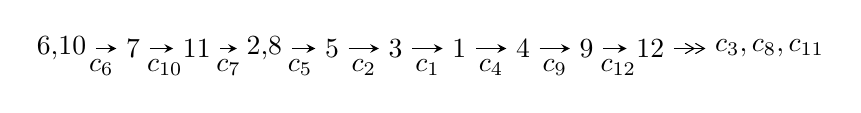
\begin{tikzpicture}[x=23pt, y=7pt]
	% node
	\node (A0) at (-1/8, 0) {6,10};
	\node (A1) at (1, 0) {7};
	\node (A2) at (2, 0) {11};
	\node (A3) at (49/16, 0) {2,8};
	\node (A4) at (33/8, 0) {5};
	\node (A5) at (41/8, 0) {3};
	\node (A6) at (49/8, 0) {1};
	\node (A7) at (57/8, 0) {4};
	\node (A8) at (65/8, 0) {9};
	\node (A9) at (73/8, 0) {12};
	\node (C1) at (1/2, -1) {$c_{6}$};
	\node (C2) at (3/2, -1) {$c_{10}$};
	\node (C3) at (5/2, -1) {$c_{7}$};
	\node (C4) at (29/8, -1) {$c_{5}$};
	\node (C5) at (37/8, -1) {$c_{2}$};
	\node (C6) at (45/8, -1) {$c_{1}$};
	\node (C7) at (53/8, -1) {$c_{4}$};
	\node (C8) at (61/8, -1) {$c_{9}$};
	\node (C9) at (69/8, -1) {$c_{12}$};
	\node (A10) at (11, 0) {$c_{3},c_{8},c_{11}$};

	% edge
	\draw[->,>=stealth]	
	(A0) edge (A1) (A1) edge (A2) (A2) edge (A3) (A3) edge (A4) (A4) edge (A5) (A5) edge (A6) (A6) edge (A7) (A7) edge (A8) (A8) edge (A9) ;
	\draw[->>,>={angle 60}]	
	(A9) edge (A10);
\end{tikzpicture} \\ 

\end{tabular} \\

\footnotetext{
The image of knot diagram is generated by the software ``\textbf{Draw programme}" developed by Andrew Bartholomew(\url{http://www.layer8.co.uk/maths/draw/index.htm\#Running-draw}), where we modified some parts for our purpose(\url{https://github.com/CATsTAILs/LinksPainter}).
}\phantom \\ \newline 
\centering \textbf{Ideals for irreducible components\footnotemark of $X_{\text{par}}$} 
 
\begin{align*}
I^u_{1}&=\langle 
-1.45180\times10^{120} u^{73}+4.03952\times10^{120} u^{72}+\cdots+1.30235\times10^{121} b-4.34074\times10^{120},\\
\phantom{I^u_{1}}&\phantom{= \langle  }6.05606\times10^{120} u^{73}-3.93278\times10^{121} u^{72}+\cdots+2.21400\times10^{122} a+2.14853\times10^{123},\\
\phantom{I^u_{1}}&\phantom{= \langle  }u^{74}-3 u^{73}+\cdots-105 u-34\rangle \\
I^u_{2}&=\langle 
b^2- b+1,\;a+1,\;u^5- u^4-2 u^3+u^2+u+1\rangle \\
\\
\end{align*}
\raggedright * 2 irreducible components of $\dim_{\mathbb{C}}=0$, with total 84 representations.\\
\footnotetext{All coefficients of polynomials are rational numbers. But the coefficients are sometimes approximated in decimal forms when there is not enough margin.}
\newpage
\renewcommand{\arraystretch}{1}
\centering \section*{I. $I^u_{1}= \langle -1.45\times10^{120} u^{73}+4.04\times10^{120} u^{72}+\cdots+1.30\times10^{121} b-4.34\times10^{120},\;6.06\times10^{120} u^{73}-3.93\times10^{121} u^{72}+\cdots+2.21\times10^{122} a+2.15\times10^{123},\;u^{74}-3 u^{73}+\cdots-105 u-34 \rangle$}
\flushleft \textbf{(i) Arc colorings}\\
\begin{tabular}{m{7pt} m{180pt} m{7pt} m{180pt} }
\flushright $a_{6}=$&$\begin{pmatrix}1\\0\end{pmatrix}$ \\
\flushright $a_{10}=$&$\begin{pmatrix}0\\u\end{pmatrix}$ \\
\flushright $a_{7}=$&$\begin{pmatrix}1\\- u^2\end{pmatrix}$ \\
\flushright $a_{11}=$&$\begin{pmatrix}u\\- u^3+u\end{pmatrix}$ \\
\flushright $a_{2}=$&$\begin{pmatrix}-0.0273534 u^{73}+0.177632 u^{72}+\cdots-9.08897 u-9.70429\\0.111475 u^{73}-0.310170 u^{72}+\cdots+0.717542 u+0.333299\end{pmatrix}$ \\
\flushright $a_{8}=$&$\begin{pmatrix}- u^2+1\\u^4-2 u^2\end{pmatrix}$ \\
\flushright $a_{5}=$&$\begin{pmatrix}0.0451659 u^{73}-0.400611 u^{72}+\cdots-29.8846 u-4.08994\\-0.0475614 u^{73}+0.362089 u^{72}+\cdots+24.0421 u+8.35798\end{pmatrix}$ \\
\flushright $a_{3}=$&$\begin{pmatrix}-0.331234 u^{73}+1.03101 u^{72}+\cdots+4.46259 u+4.44330\\0.239159 u^{73}-0.574819 u^{72}+\cdots-2.80721 u-9.58086\end{pmatrix}$ \\
\flushright $a_{1}=$&$\begin{pmatrix}-0.210920 u^{73}+0.849732 u^{72}+\cdots+23.6544 u+14.0350\\-0.147525 u^{73}+0.442629 u^{72}+\cdots+7.67513 u+1.20613\end{pmatrix}$ \\
\flushright $a_{4}=$&$\begin{pmatrix}-0.00239555 u^{73}-0.0385226 u^{72}+\cdots-5.84249 u+4.26805\\-0.0475614 u^{73}+0.362089 u^{72}+\cdots+24.0421 u+8.35798\end{pmatrix}$ \\
\flushright $a_{9}=$&$\begin{pmatrix}-0.0354744 u^{73}+0.253948 u^{72}+\cdots+6.90667 u-3.95032\\0.217027 u^{73}-0.765655 u^{72}+\cdots-22.3956 u-12.1871\end{pmatrix}$ \\
\flushright $a_{12}=$&$\begin{pmatrix}-0.361662 u^{73}+1.35032 u^{72}+\cdots+39.2427 u+19.9087\\-0.0399039 u^{73}+0.190967 u^{72}+\cdots+4.64937 u-3.21561\end{pmatrix}$\\&\end{tabular}
\flushleft \textbf{(ii) Obstruction class $= -1$}\\~\\
\flushleft \textbf{(iii) Cusp Shapes $= -0.0808785 u^{73}+0.245428 u^{72}+\cdots-15.6772 u-2.16608$}\\~\\
\newpage\renewcommand{\arraystretch}{1}
\flushleft \textbf{(iv) u-Polynomials at the component}\newline \\
\begin{tabular}{m{50pt}|m{274pt}}
Crossings & \hspace{64pt}u-Polynomials at each crossing \\
\hline $$\begin{aligned}c_{1},c_{4}\end{aligned}$$&$\begin{aligned}
&u^{74}+22 u^{73}+\cdots+13 u+1
\end{aligned}$\\
\hline $$\begin{aligned}c_{2},c_{5}\end{aligned}$$&$\begin{aligned}
&u^{74}+6 u^{73}+\cdots+5 u+1
\end{aligned}$\\
\hline $$\begin{aligned}c_{3},c_{9}\end{aligned}$$&$\begin{aligned}
&u^{74}+u^{73}+\cdots+3072 u^2-1024
\end{aligned}$\\
\hline $$\begin{aligned}c_{6},c_{7},c_{10}\end{aligned}$$&$\begin{aligned}
&u^{74}-3 u^{73}+\cdots-105 u-34
\end{aligned}$\\
\hline $$\begin{aligned}c_{8},c_{12}\end{aligned}$$&$\begin{aligned}
&u^{74}+3 u^{73}+\cdots-2 u-1
\end{aligned}$\\
\hline $$\begin{aligned}c_{11}\end{aligned}$$&$\begin{aligned}
&u^{74}-43 u^{73}+\cdots+2 u+1
\end{aligned}$\\
\hline
\end{tabular}\\~\\
\newpage\renewcommand{\arraystretch}{1}
\flushleft \textbf{(v) Riley Polynomials at the component}\newline \\
\begin{tabular}{m{50pt}|m{274pt}}
Crossings & \hspace{64pt}Riley Polynomials at each crossing \\
\hline $$\begin{aligned}c_{1},c_{4}\end{aligned}$$&$\begin{aligned}
&y^{74}+66 y^{73}+\cdots+1221 y+1
\end{aligned}$\\
\hline $$\begin{aligned}c_{2},c_{5}\end{aligned}$$&$\begin{aligned}
&y^{74}+22 y^{73}+\cdots+13 y+1
\end{aligned}$\\
\hline $$\begin{aligned}c_{3},c_{9}\end{aligned}$$&$\begin{aligned}
&y^{74}-55 y^{73}+\cdots-6291456 y+1048576
\end{aligned}$\\
\hline $$\begin{aligned}c_{6},c_{7},c_{10}\end{aligned}$$&$\begin{aligned}
&y^{74}-85 y^{73}+\cdots+17603 y+1156
\end{aligned}$\\
\hline $$\begin{aligned}c_{8},c_{12}\end{aligned}$$&$\begin{aligned}
&y^{74}+43 y^{73}+\cdots-2 y+1
\end{aligned}$\\
\hline $$\begin{aligned}c_{11}\end{aligned}$$&$\begin{aligned}
&y^{74}-21 y^{73}+\cdots-54 y+1
\end{aligned}$\\
\hline
\end{tabular}\\~\\
\newpage\flushleft \textbf{(vi) Complex Volumes and Cusp Shapes}
$$\begin{array}{c|c|c}  
\text{Solutions to }I^u_{1}& \I (\text{vol} + \sqrt{-1}CS) & \text{Cusp shape}\\
 \hline 
\begin{aligned}
u &= -0.792276 + 0.579163 I \\
a &= -0.405399 - 0.850260 I \\
b &= \phantom{-}0.218212 - 1.039340 I\end{aligned}
 & \phantom{-}0.15163 - 5.92978 I & \phantom{-0.000000 } 0 \\ \hline\begin{aligned}
u &= -0.792276 - 0.579163 I \\
a &= -0.405399 + 0.850260 I \\
b &= \phantom{-}0.218212 + 1.039340 I\end{aligned}
 & \phantom{-}0.15163 + 5.92978 I & \phantom{-0.000000 } 0 \\ \hline\begin{aligned}
u &= \phantom{-}0.141074 + 1.026160 I \\
a &= \phantom{-}0.741246 - 0.573106 I \\
b &= -0.754093 - 0.901400 I\end{aligned}
 & \phantom{-}2.82540 + 5.08946 I & \phantom{-0.000000 } 0 \\ \hline\begin{aligned}
u &= \phantom{-}0.141074 - 1.026160 I \\
a &= \phantom{-}0.741246 + 0.573106 I \\
b &= -0.754093 + 0.901400 I\end{aligned}
 & \phantom{-}2.82540 - 5.08946 I & \phantom{-0.000000 } 0 \\ \hline\begin{aligned}
u &= \phantom{-}0.247837 + 1.018910 I \\
a &= \phantom{-}0.476613 + 0.271184 I \\
b &= -0.759452 + 0.862977 I\end{aligned}
 & \phantom{-}2.94401 - 0.64407 I & \phantom{-0.000000 } 0 \\ \hline\begin{aligned}
u &= \phantom{-}0.247837 - 1.018910 I \\
a &= \phantom{-}0.476613 - 0.271184 I \\
b &= -0.759452 - 0.862977 I\end{aligned}
 & \phantom{-}2.94401 + 0.64407 I & \phantom{-0.000000 } 0 \\ \hline\begin{aligned}
u &= \phantom{-}0.738891 + 0.770167 I \\
a &= \phantom{-}1.42413 - 0.69452 I \\
b &= -0.768564 - 0.958680 I\end{aligned}
 & \phantom{-}4.37578 + 6.45349 I & \phantom{-0.000000 } 0 \\ \hline\begin{aligned}
u &= \phantom{-}0.738891 - 0.770167 I \\
a &= \phantom{-}1.42413 + 0.69452 I \\
b &= -0.768564 + 0.958680 I\end{aligned}
 & \phantom{-}4.37578 - 6.45349 I & \phantom{-0.000000 } 0 \\ \hline\begin{aligned}
u &= \phantom{-}0.819080 + 0.694478 I \\
a &= \phantom{-}0.395577 - 0.433900 I \\
b &= -0.809713 + 0.803977 I\end{aligned}
 & \phantom{-}4.85168 + 0.52465 I & \phantom{-0.000000 } 0 \\ \hline\begin{aligned}
u &= \phantom{-}0.819080 - 0.694478 I \\
a &= \phantom{-}0.395577 + 0.433900 I \\
b &= -0.809713 - 0.803977 I\end{aligned}
 & \phantom{-}4.85168 - 0.52465 I & \phantom{-0.000000 } 0\\
 \hline 
 \end{array}$$\newpage$$\begin{array}{c|c|c}  
\text{Solutions to }I^u_{1}& \I (\text{vol} + \sqrt{-1}CS) & \text{Cusp shape}\\
 \hline 
\begin{aligned}
u &= \phantom{-}0.833315 + 0.399088 I \\
a &= -2.05047 - 0.63615 I \\
b &= \phantom{-}0.684280 + 0.914822 I\end{aligned}
 & \phantom{-}2.91943 + 5.78714 I & \phantom{-0.000000 } 0 \\ \hline\begin{aligned}
u &= \phantom{-}0.833315 - 0.399088 I \\
a &= -2.05047 + 0.63615 I \\
b &= \phantom{-}0.684280 - 0.914822 I\end{aligned}
 & \phantom{-}2.91943 - 5.78714 I & \phantom{-0.000000 } 0 \\ \hline\begin{aligned}
u &= -0.833568 + 0.293621 I \\
a &= -0.491785 + 0.392953 I \\
b &= \phantom{-}0.641432 - 0.143331 I\end{aligned}
 & \phantom{-}3.80185 - 3.25281 I & \phantom{-}12.99162 + 5.07017 I \\ \hline\begin{aligned}
u &= -0.833568 - 0.293621 I \\
a &= -0.491785 - 0.392953 I \\
b &= \phantom{-}0.641432 + 0.143331 I\end{aligned}
 & \phantom{-}3.80185 + 3.25281 I & \phantom{-}12.99162 - 5.07017 I \\ \hline\begin{aligned}
u &= \phantom{-}0.536029 + 0.688679 I \\
a &= \phantom{-}1.157520 - 0.586197 I \\
b &= -0.016192 - 0.798494 I\end{aligned}
 & -1.03766 + 2.07310 I & \phantom{-0.000000 } 0. - 3.44701 I \\ \hline\begin{aligned}
u &= \phantom{-}0.536029 - 0.688679 I \\
a &= \phantom{-}1.157520 + 0.586197 I \\
b &= -0.016192 + 0.798494 I\end{aligned}
 & -1.03766 - 2.07310 I & \phantom{-0.000000 -}0. + 3.44701 I \\ \hline\begin{aligned}
u &= \phantom{-}0.749591 + 0.262619 I \\
a &= -2.06221 + 0.99351 I \\
b &= \phantom{-}0.705257 - 0.788110 I\end{aligned}
 & \phantom{-}3.31170 + 0.45778 I & \phantom{-}9.93937 - 0.85994 I \\ \hline\begin{aligned}
u &= \phantom{-}0.749591 - 0.262619 I \\
a &= -2.06221 - 0.99351 I \\
b &= \phantom{-}0.705257 + 0.788110 I\end{aligned}
 & \phantom{-}3.31170 - 0.45778 I & \phantom{-}9.93937 + 0.85994 I \\ \hline\begin{aligned}
u &= \phantom{-}1.273940 + 0.124542 I \\
a &= \phantom{-}1.174220 - 0.094574 I \\
b &= -0.227543 - 0.656454 I\end{aligned}
 & \phantom{-}2.04447 + 1.01310 I & \phantom{-0.000000 } 0 \\ \hline\begin{aligned}
u &= \phantom{-}1.273940 - 0.124542 I \\
a &= \phantom{-}1.174220 + 0.094574 I \\
b &= -0.227543 + 0.656454 I\end{aligned}
 & \phantom{-}2.04447 - 1.01310 I & \phantom{-0.000000 } 0\\
 \hline 
 \end{array}$$\newpage$$\begin{array}{c|c|c}  
\text{Solutions to }I^u_{1}& \I (\text{vol} + \sqrt{-1}CS) & \text{Cusp shape}\\
 \hline 
\begin{aligned}
u &= -1.059070 + 0.761879 I \\
a &= \phantom{-}1.57349 + 0.43998 I \\
b &= -0.764665 + 0.986007 I\end{aligned}
 & \phantom{-}6.38008 - 11.03360 I & \phantom{-0.000000 } 0 \\ \hline\begin{aligned}
u &= -1.059070 - 0.761879 I \\
a &= \phantom{-}1.57349 - 0.43998 I \\
b &= -0.764665 - 0.986007 I\end{aligned}
 & \phantom{-}6.38008 + 11.03360 I & \phantom{-0.000000 } 0 \\ \hline\begin{aligned}
u &= -0.645813 + 0.255567 I \\
a &= -0.114178 + 1.091410 I \\
b &= -0.851584 - 0.841956 I\end{aligned}
 & \phantom{-}9.27124 + 2.13858 I & \phantom{-}13.72041 - 2.59497 I \\ \hline\begin{aligned}
u &= -0.645813 - 0.255567 I \\
a &= -0.114178 - 1.091410 I \\
b &= -0.851584 + 0.841956 I\end{aligned}
 & \phantom{-}9.27124 - 2.13858 I & \phantom{-}13.72041 + 2.59497 I \\ \hline\begin{aligned}
u &= -1.113290 + 0.685903 I \\
a &= \phantom{-}0.659749 + 0.554990 I \\
b &= -0.825354 - 0.765471 I\end{aligned}
 & \phantom{-}7.05334 - 5.07352 I & \phantom{-0.000000 } 0 \\ \hline\begin{aligned}
u &= -1.113290 - 0.685903 I \\
a &= \phantom{-}0.659749 - 0.554990 I \\
b &= -0.825354 + 0.765471 I\end{aligned}
 & \phantom{-}7.05334 + 5.07352 I & \phantom{-0.000000 } 0 \\ \hline\begin{aligned}
u &= -0.089649 + 0.672839 I \\
a &= \phantom{-}0.88456 + 1.13933 I \\
b &= \phantom{-}0.095134 + 0.862320 I\end{aligned}
 & -1.96073 + 1.64413 I & -2.06231 - 4.26426 I \\ \hline\begin{aligned}
u &= -0.089649 - 0.672839 I \\
a &= \phantom{-}0.88456 - 1.13933 I \\
b &= \phantom{-}0.095134 - 0.862320 I\end{aligned}
 & -1.96073 - 1.64413 I & -2.06231 + 4.26426 I \\ \hline\begin{aligned}
u &= \phantom{-}0.358555 + 0.536553 I \\
a &= -0.04644 + 1.41724 I \\
b &= \phantom{-}0.197597 + 0.943333 I\end{aligned}
 & -1.56670 + 2.15882 I & -0.36505 - 4.88726 I \\ \hline\begin{aligned}
u &= \phantom{-}0.358555 - 0.536553 I \\
a &= -0.04644 - 1.41724 I \\
b &= \phantom{-}0.197597 - 0.943333 I\end{aligned}
 & -1.56670 - 2.15882 I & -0.36505 + 4.88726 I\\
 \hline 
 \end{array}$$\newpage$$\begin{array}{c|c|c}  
\text{Solutions to }I^u_{1}& \I (\text{vol} + \sqrt{-1}CS) & \text{Cusp shape}\\
 \hline 
\begin{aligned}
u &= -0.545628 + 0.285450 I \\
a &= \phantom{-}2.12519 + 1.41592 I \\
b &= -0.813472 + 0.950753 I\end{aligned}
 & \phantom{-}8.93340 - 4.05613 I & \phantom{-}13.18636 + 2.67213 I \\ \hline\begin{aligned}
u &= -0.545628 - 0.285450 I \\
a &= \phantom{-}2.12519 - 1.41592 I \\
b &= -0.813472 - 0.950753 I\end{aligned}
 & \phantom{-}8.93340 + 4.05613 I & \phantom{-}13.18636 - 2.67213 I \\ \hline\begin{aligned}
u &= -0.538990 + 0.296954 I \\
a &= -1.66267 + 0.63971 I \\
b &= \phantom{-}0.413810 + 1.006280 I\end{aligned}
 & \phantom{-}1.269800 + 0.465685 I & \phantom{-}10.92617 + 0.56708 I \\ \hline\begin{aligned}
u &= -0.538990 - 0.296954 I \\
a &= -1.66267 - 0.63971 I \\
b &= \phantom{-}0.413810 - 1.006280 I\end{aligned}
 & \phantom{-}1.269800 - 0.465685 I & \phantom{-}10.92617 - 0.56708 I \\ \hline\begin{aligned}
u &= -1.392270 + 0.138352 I \\
a &= \phantom{-}1.157120 - 0.037316 I \\
b &= -0.289785 - 0.621402 I\end{aligned}
 & \phantom{-}5.70309 - 3.30850 I & \phantom{-0.000000 } 0 \\ \hline\begin{aligned}
u &= -1.392270 - 0.138352 I \\
a &= \phantom{-}1.157120 + 0.037316 I \\
b &= -0.289785 + 0.621402 I\end{aligned}
 & \phantom{-}5.70309 + 3.30850 I & \phantom{-0.000000 } 0 \\ \hline\begin{aligned}
u &= \phantom{-}0.590098\phantom{ +0.000000I} \\
a &= \phantom{-}0.115562\phantom{ +0.000000I} \\
b &= \phantom{-}0.437328\phantom{ +0.000000I}\end{aligned}
 & \phantom{-}1.09942\phantom{ +0.000000I} & \phantom{-}9.14060\phantom{ +0.000000I} \\ \hline\begin{aligned}
u &= \phantom{-}0.275924 + 0.441037 I \\
a &= \phantom{-}1.129560 - 0.072563 I \\
b &= -0.142548 + 0.140247 I\end{aligned}
 & \phantom{-}0.50148 + 1.32272 I & \phantom{-}5.11712 - 4.95919 I \\ \hline\begin{aligned}
u &= \phantom{-}0.275924 - 0.441037 I \\
a &= \phantom{-}1.129560 + 0.072563 I \\
b &= -0.142548 - 0.140247 I\end{aligned}
 & \phantom{-}0.50148 - 1.32272 I & \phantom{-}5.11712 + 4.95919 I \\ \hline\begin{aligned}
u &= -1.48500 + 0.26000 I \\
a &= \phantom{-}1.120910 + 0.102882 I \\
b &= -0.255453 + 0.705274 I\end{aligned}
 & \phantom{-}5.45005 - 5.59065 I & \phantom{-0.000000 } 0\\
 \hline 
 \end{array}$$\newpage$$\begin{array}{c|c|c}  
\text{Solutions to }I^u_{1}& \I (\text{vol} + \sqrt{-1}CS) & \text{Cusp shape}\\
 \hline 
\begin{aligned}
u &= -1.48500 - 0.26000 I \\
a &= \phantom{-}1.120910 - 0.102882 I \\
b &= -0.255453 - 0.705274 I\end{aligned}
 & \phantom{-}5.45005 + 5.59065 I & \phantom{-0.000000 } 0 \\ \hline\begin{aligned}
u &= -0.463679 + 0.155250 I \\
a &= -2.37623 + 0.65762 I \\
b &= \phantom{-}0.614271 - 0.862447 I\end{aligned}
 & \phantom{-}0.59794 - 2.40390 I & \phantom{-}1.78729 + 3.32649 I \\ \hline\begin{aligned}
u &= -0.463679 - 0.155250 I \\
a &= -2.37623 - 0.65762 I \\
b &= \phantom{-}0.614271 + 0.862447 I\end{aligned}
 & \phantom{-}0.59794 + 2.40390 I & \phantom{-}1.78729 - 3.32649 I \\ \hline\begin{aligned}
u &= -1.51959 + 0.08438 I \\
a &= -0.789869 - 0.291182 I \\
b &= \phantom{-}0.306865 - 1.151720 I\end{aligned}
 & \phantom{-}4.67990 - 3.98112 I & \phantom{-0.000000 } 0 \\ \hline\begin{aligned}
u &= -1.51959 - 0.08438 I \\
a &= -0.789869 + 0.291182 I \\
b &= \phantom{-}0.306865 + 1.151720 I\end{aligned}
 & \phantom{-}4.67990 + 3.98112 I & \phantom{-0.000000 } 0 \\ \hline\begin{aligned}
u &= -0.078329 + 0.427211 I \\
a &= -2.27926 + 0.07772 I \\
b &= \phantom{-}0.541612 - 0.940323 I\end{aligned}
 & \phantom{-}0.26280 - 2.86416 I & \phantom{-}5.10786 - 1.03407 I \\ \hline\begin{aligned}
u &= -0.078329 - 0.427211 I \\
a &= -2.27926 - 0.07772 I \\
b &= \phantom{-}0.541612 + 0.940323 I\end{aligned}
 & \phantom{-}0.26280 + 2.86416 I & \phantom{-}5.10786 + 1.03407 I \\ \hline\begin{aligned}
u &= \phantom{-}1.56928 + 0.03188 I \\
a &= -1.87634 - 0.78270 I \\
b &= \phantom{-}0.803759 + 0.892022 I\end{aligned}
 & \phantom{-}7.70040 + 3.01101 I & \phantom{-0.000000 } 0 \\ \hline\begin{aligned}
u &= \phantom{-}1.56928 - 0.03188 I \\
a &= -1.87634 + 0.78270 I \\
b &= \phantom{-}0.803759 - 0.892022 I\end{aligned}
 & \phantom{-}7.70040 - 3.01101 I & \phantom{-0.000000 } 0 \\ \hline\begin{aligned}
u &= \phantom{-}1.57468 + 0.06012 I \\
a &= -0.847918 - 0.235707 I \\
b &= \phantom{-}0.325364 - 1.160820 I\end{aligned}
 & \phantom{-}8.54134 + 0.68666 I & \phantom{-0.000000 } 0\\
 \hline 
 \end{array}$$\newpage$$\begin{array}{c|c|c}  
\text{Solutions to }I^u_{1}& \I (\text{vol} + \sqrt{-1}CS) & \text{Cusp shape}\\
 \hline 
\begin{aligned}
u &= \phantom{-}1.57468 - 0.06012 I \\
a &= -0.847918 + 0.235707 I \\
b &= \phantom{-}0.325364 + 1.160820 I\end{aligned}
 & \phantom{-}8.54134 - 0.68666 I & \phantom{-0.000000 } 0 \\ \hline\begin{aligned}
u &= -1.58471\phantom{ +0.000000I} \\
a &= -0.992474\phantom{ +0.000000I} \\
b &= \phantom{-}0.861914\phantom{ +0.000000I}\end{aligned}
 & \phantom{-}8.58805\phantom{ +0.000000I} & \phantom{-0.000000 } 0 \\ \hline\begin{aligned}
u &= \phantom{-}1.58785 + 0.09233 I \\
a &= \phantom{-}1.94370 + 0.00627 I \\
b &= -0.811458 - 1.037490 I\end{aligned}
 & \phantom{-}16.3498 + 5.4804 I & \phantom{-0.000000 } 0 \\ \hline\begin{aligned}
u &= \phantom{-}1.58785 - 0.09233 I \\
a &= \phantom{-}1.94370 - 0.00627 I \\
b &= -0.811458 + 1.037490 I\end{aligned}
 & \phantom{-}16.3498 - 5.4804 I & \phantom{-0.000000 } 0 \\ \hline\begin{aligned}
u &= \phantom{-}1.62114 + 0.06754 I \\
a &= \phantom{-}1.07652 - 0.93449 I \\
b &= -0.933998 + 0.760204 I\end{aligned}
 & \phantom{-}17.2245 - 0.9450 I & \phantom{-0.000000 } 0 \\ \hline\begin{aligned}
u &= \phantom{-}1.62114 - 0.06754 I \\
a &= \phantom{-}1.07652 + 0.93449 I \\
b &= -0.933998 - 0.760204 I\end{aligned}
 & \phantom{-}17.2245 + 0.9450 I & \phantom{-0.000000 } 0 \\ \hline\begin{aligned}
u &= -1.62817 + 0.07722 I \\
a &= -1.86464 - 0.79697 I \\
b &= \phantom{-}0.816768 + 0.882730 I\end{aligned}
 & \phantom{-}11.54420 - 1.76278 I & \phantom{-0.000000 } 0 \\ \hline\begin{aligned}
u &= -1.62817 - 0.07722 I \\
a &= -1.86464 + 0.79697 I \\
b &= \phantom{-}0.816768 - 0.882730 I\end{aligned}
 & \phantom{-}11.54420 + 1.76278 I & \phantom{-0.000000 } 0 \\ \hline\begin{aligned}
u &= -1.62013 + 0.22649 I \\
a &= \phantom{-}1.87179 + 0.02364 I \\
b &= -0.800729 + 1.038330 I\end{aligned}
 & \phantom{-}12.2115 - 10.1477 I & \phantom{-0.000000 } 0 \\ \hline\begin{aligned}
u &= -1.62013 - 0.22649 I \\
a &= \phantom{-}1.87179 - 0.02364 I \\
b &= -0.800729 - 1.038330 I\end{aligned}
 & \phantom{-}12.2115 + 10.1477 I & \phantom{-0.000000 } 0\\
 \hline 
 \end{array}$$\newpage$$\begin{array}{c|c|c}  
\text{Solutions to }I^u_{1}& \I (\text{vol} + \sqrt{-1}CS) & \text{Cusp shape}\\
 \hline 
\begin{aligned}
u &= \phantom{-}1.63229 + 0.17241 I \\
a &= -0.729730 + 0.249243 I \\
b &= \phantom{-}0.294541 + 1.166160 I\end{aligned}
 & \phantom{-}8.34692 + 8.79923 I & \phantom{-0.000000 } 0 \\ \hline\begin{aligned}
u &= \phantom{-}1.63229 - 0.17241 I \\
a &= -0.729730 - 0.249243 I \\
b &= \phantom{-}0.294541 - 1.166160 I\end{aligned}
 & \phantom{-}8.34692 - 8.79923 I & \phantom{-0.000000 } 0 \\ \hline\begin{aligned}
u &= -1.64023 + 0.18527 I \\
a &= \phantom{-}1.055260 + 0.872816 I \\
b &= -0.925763 - 0.748096 I\end{aligned}
 & \phantom{-}13.12460 - 3.78419 I & \phantom{-0.000000 } 0 \\ \hline\begin{aligned}
u &= -1.64023 - 0.18527 I \\
a &= \phantom{-}1.055260 - 0.872816 I \\
b &= -0.925763 + 0.748096 I\end{aligned}
 & \phantom{-}13.12460 + 3.78419 I & \phantom{-0.000000 } 0 \\ \hline\begin{aligned}
u &= \phantom{-}1.64954 + 0.09451 I \\
a &= -1.024770 - 0.042625 I \\
b &= \phantom{-}0.877470 + 0.021197 I\end{aligned}
 & \phantom{-}12.40730 + 4.81921 I & \phantom{-0.000000 } 0 \\ \hline\begin{aligned}
u &= \phantom{-}1.64954 - 0.09451 I \\
a &= -1.024770 + 0.042625 I \\
b &= \phantom{-}0.877470 - 0.021197 I\end{aligned}
 & \phantom{-}12.40730 - 4.81921 I & \phantom{-0.000000 } 0 \\ \hline\begin{aligned}
u &= -1.64916 + 0.12208 I \\
a &= -1.86517 + 0.76861 I \\
b &= \phantom{-}0.808404 - 0.906622 I\end{aligned}
 & \phantom{-}11.46920 - 7.83965 I & \phantom{-0.000000 } 0 \\ \hline\begin{aligned}
u &= -1.64916 - 0.12208 I \\
a &= -1.86517 - 0.76861 I \\
b &= \phantom{-}0.808404 + 0.906622 I\end{aligned}
 & \phantom{-}11.46920 + 7.83965 I & \phantom{-0.000000 } 0 \\ \hline\begin{aligned}
u &= \phantom{-}0.011633 + 0.252597 I \\
a &= -1.48519 - 3.25207 I \\
b &= \phantom{-}0.486901 + 0.619078 I\end{aligned}
 & \phantom{-}1.18181 + 1.37684 I & \phantom{-}10.23383 - 4.11434 I \\ \hline\begin{aligned}
u &= \phantom{-}0.011633 - 0.252597 I \\
a &= -1.48519 + 3.25207 I \\
b &= \phantom{-}0.486901 - 0.619078 I\end{aligned}
 & \phantom{-}1.18181 - 1.37684 I & \phantom{-}10.23383 + 4.11434 I\\
 \hline 
 \end{array}$$\newpage$$\begin{array}{c|c|c}  
\text{Solutions to }I^u_{1}& \I (\text{vol} + \sqrt{-1}CS) & \text{Cusp shape}\\
 \hline 
\begin{aligned}
u &= \phantom{-}1.73327 + 0.24468 I \\
a &= \phantom{-}1.83247 + 0.02129 I \\
b &= -0.798044 - 1.046890 I\end{aligned}
 & \phantom{-}15.8035 + 15.1907 I & \phantom{-0.000000 } 0 \\ \hline\begin{aligned}
u &= \phantom{-}1.73327 - 0.24468 I \\
a &= \phantom{-}1.83247 - 0.02129 I \\
b &= -0.798044 + 1.046890 I\end{aligned}
 & \phantom{-}15.8035 - 15.1907 I & \phantom{-0.000000 } 0 \\ \hline\begin{aligned}
u &= \phantom{-}1.73825 + 0.21069 I \\
a &= \phantom{-}1.096380 - 0.840577 I \\
b &= -0.932887 + 0.737413 I\end{aligned}
 & \phantom{-}16.7780 + 8.8164 I & \phantom{-0.000000 } 0 \\ \hline\begin{aligned}
u &= \phantom{-}1.73825 - 0.21069 I \\
a &= \phantom{-}1.096380 + 0.840577 I \\
b &= -0.932887 - 0.737413 I\end{aligned}
 & \phantom{-}16.7780 - 8.8164 I & \phantom{-0.000000 } 0\\
 \hline 
 \end{array}$$\newpage\newpage\renewcommand{\arraystretch}{1}
\centering \section*{II. $I^u_{2}= \langle b^2- b+1,\;a+1,\;u^5- u^4-2 u^3+u^2+u+1 \rangle$}
\flushleft \textbf{(i) Arc colorings}\\
\begin{tabular}{m{7pt} m{180pt} m{7pt} m{180pt} }
\flushright $a_{6}=$&$\begin{pmatrix}1\\0\end{pmatrix}$ \\
\flushright $a_{10}=$&$\begin{pmatrix}0\\u\end{pmatrix}$ \\
\flushright $a_{7}=$&$\begin{pmatrix}1\\- u^2\end{pmatrix}$ \\
\flushright $a_{11}=$&$\begin{pmatrix}u\\- u^3+u\end{pmatrix}$ \\
\flushright $a_{2}=$&$\begin{pmatrix}-1\\b\end{pmatrix}$ \\
\flushright $a_{8}=$&$\begin{pmatrix}- u^2+1\\u^4-2 u^2\end{pmatrix}$ \\
\flushright $a_{5}=$&$\begin{pmatrix}- b+1\\b-1\end{pmatrix}$ \\
\flushright $a_{3}=$&$\begin{pmatrix}0\\b-1\end{pmatrix}$ \\
\flushright $a_{1}=$&$\begin{pmatrix}-1\\0\end{pmatrix}$ \\
\flushright $a_{4}=$&$\begin{pmatrix}0\\b-1\end{pmatrix}$ \\
\flushright $a_{9}=$&$\begin{pmatrix}0\\u\end{pmatrix}$ \\
\flushright $a_{12}=$&$\begin{pmatrix}- u^3+2 u\\- u^3+u\end{pmatrix}$\\&\end{tabular}
\flushleft \textbf{(ii) Obstruction class $= 1$}\\~\\
\flushleft \textbf{(iii) Cusp Shapes $= u^4 b-2 u^3 b-2 u^2 b-4 u^3+3 b u+u^2-4 b+8 u+10$}\\~\\
\newpage\renewcommand{\arraystretch}{1}
\flushleft \textbf{(iv) u-Polynomials at the component}\newline \\
\begin{tabular}{m{50pt}|m{274pt}}
Crossings & \hspace{64pt}u-Polynomials at each crossing \\
\hline $$\begin{aligned}c_{1},c_{4},c_{5}\end{aligned}$$&$\begin{aligned}
&(u^2- u+1)^5
\end{aligned}$\\
\hline $$\begin{aligned}c_{2}\end{aligned}$$&$\begin{aligned}
&(u^2+u+1)^5
\end{aligned}$\\
\hline $$\begin{aligned}c_{3},c_{9}\end{aligned}$$&$\begin{aligned}
&u^{10}
\end{aligned}$\\
\hline $$\begin{aligned}c_{6},c_{7}\end{aligned}$$&$\begin{aligned}
&(u^5- u^4-2 u^3+u^2+u+1)^2
\end{aligned}$\\
\hline $$\begin{aligned}c_{8}\end{aligned}$$&$\begin{aligned}
&(u^5+u^4+2 u^3+u^2+u+1)^2
\end{aligned}$\\
\hline $$\begin{aligned}c_{10}\end{aligned}$$&$\begin{aligned}
&(u^5+u^4-2 u^3- u^2+u-1)^2
\end{aligned}$\\
\hline $$\begin{aligned}c_{11}\end{aligned}$$&$\begin{aligned}
&(u^5+3 u^4+4 u^3+u^2- u-1)^2
\end{aligned}$\\
\hline $$\begin{aligned}c_{12}\end{aligned}$$&$\begin{aligned}
&(u^5- u^4+2 u^3- u^2+u-1)^2
\end{aligned}$\\
\hline
\end{tabular}\\~\\
\newpage\renewcommand{\arraystretch}{1}
\flushleft \textbf{(v) Riley Polynomials at the component}\newline \\
\begin{tabular}{m{50pt}|m{274pt}}
Crossings & \hspace{64pt}Riley Polynomials at each crossing \\
\hline $$\begin{aligned}c_{1},c_{2},c_{4}\\c_{5}\end{aligned}$$&$\begin{aligned}
&(y^2+y+1)^5
\end{aligned}$\\
\hline $$\begin{aligned}c_{3},c_{9}\end{aligned}$$&$\begin{aligned}
&y^{10}
\end{aligned}$\\
\hline $$\begin{aligned}c_{6},c_{7},c_{10}\end{aligned}$$&$\begin{aligned}
&(y^5-5 y^4+8 y^3-3 y^2- y-1)^2
\end{aligned}$\\
\hline $$\begin{aligned}c_{8},c_{12}\end{aligned}$$&$\begin{aligned}
&(y^5+3 y^4+4 y^3+y^2- y-1)^2
\end{aligned}$\\
\hline $$\begin{aligned}c_{11}\end{aligned}$$&$\begin{aligned}
&(y^5- y^4+8 y^3-3 y^2+3 y-1)^2
\end{aligned}$\\
\hline
\end{tabular}\\~\\
\newpage\flushleft \textbf{(vi) Complex Volumes and Cusp Shapes}
$$\begin{array}{c|c|c}  
\text{Solutions to }I^u_{2}& \I (\text{vol} + \sqrt{-1}CS) & \text{Cusp shape}\\
 \hline 
\begin{aligned}
u &= -1.21774\phantom{ +0.000000I} \\
a &= -1.00000\phantom{ +0.000000I} \\
b &= \phantom{-}0.500000 + 0.866025 I\end{aligned}
 & \phantom{-}2.40108 + 2.02988 I & \phantom{-}6.55976 - 4.16430 I \\ \hline\begin{aligned}
u &= -1.21774\phantom{ +0.000000I} \\
a &= -1.00000\phantom{ +0.000000I} \\
b &= \phantom{-}0.500000 - 0.866025 I\end{aligned}
 & \phantom{-}2.40108 - 2.02988 I & \phantom{-}6.55976 + 4.16430 I \\ \hline\begin{aligned}
u &= -0.309916 + 0.549911 I \\
a &= -1.00000\phantom{ +0.000000I} \\
b &= \phantom{-}0.500000 + 0.866025 I\end{aligned}
 & \phantom{-}0.329100 + 0.499304 I & \phantom{-}1.60756 + 0.92266 I \\ \hline\begin{aligned}
u &= -0.309916 + 0.549911 I \\
a &= -1.00000\phantom{ +0.000000I} \\
b &= \phantom{-}0.500000 - 0.866025 I\end{aligned}
 & \phantom{-}0.32910 - 3.56046 I & \phantom{-}5.91654 + 9.74472 I \\ \hline\begin{aligned}
u &= -0.309916 - 0.549911 I \\
a &= -1.00000\phantom{ +0.000000I} \\
b &= \phantom{-}0.500000 + 0.866025 I\end{aligned}
 & \phantom{-}0.32910 + 3.56046 I & \phantom{-}5.91654 - 9.74472 I \\ \hline\begin{aligned}
u &= -0.309916 - 0.549911 I \\
a &= -1.00000\phantom{ +0.000000I} \\
b &= \phantom{-}0.500000 - 0.866025 I\end{aligned}
 & \phantom{-}0.329100 - 0.499304 I & \phantom{-}1.60756 - 0.92266 I \\ \hline\begin{aligned}
u &= \phantom{-}1.41878 + 0.21917 I \\
a &= -1.00000\phantom{ +0.000000I} \\
b &= \phantom{-}0.500000 + 0.866025 I\end{aligned}
 & \phantom{-}5.87256 + 6.43072 I & \phantom{-}10.62344 - 8.02599 I \\ \hline\begin{aligned}
u &= \phantom{-}1.41878 + 0.21917 I \\
a &= -1.00000\phantom{ +0.000000I} \\
b &= \phantom{-}0.500000 - 0.866025 I\end{aligned}
 & \phantom{-}5.87256 + 2.37095 I & \phantom{-}9.29269 + 1.50431 I \\ \hline\begin{aligned}
u &= \phantom{-}1.41878 - 0.21917 I \\
a &= -1.00000\phantom{ +0.000000I} \\
b &= \phantom{-}0.500000 + 0.866025 I\end{aligned}
 & \phantom{-}5.87256 - 2.37095 I & \phantom{-}9.29269 - 1.50431 I \\ \hline\begin{aligned}
u &= \phantom{-}1.41878 - 0.21917 I \\
a &= -1.00000\phantom{ +0.000000I} \\
b &= \phantom{-}0.500000 - 0.866025 I\end{aligned}
 & \phantom{-}5.87256 - 6.43072 I & \phantom{-}10.62344 + 8.02599 I\\
 \hline 
 \end{array}$$\newpage
\newpage\renewcommand{\arraystretch}{1}
\centering \section*{ III. u-Polynomials}
\begin{tabular}{m{50pt}|m{274pt}}
Crossings & \hspace{64pt}u-Polynomials at each crossing \\
\hline $$\begin{aligned}c_{1},c_{4}\end{aligned}$$&$\begin{aligned}
&((u^2- u+1)^5)(u^{74}+22 u^{73}+\cdots+13 u+1)
\end{aligned}$\\
\hline $$\begin{aligned}c_{2}\end{aligned}$$&$\begin{aligned}
&((u^2+u+1)^5)(u^{74}+6 u^{73}+\cdots+5 u+1)
\end{aligned}$\\
\hline $$\begin{aligned}c_{3},c_{9}\end{aligned}$$&$\begin{aligned}
&u^{10}(u^{74}+u^{73}+\cdots+3072 u^2-1024)
\end{aligned}$\\
\hline $$\begin{aligned}c_{5}\end{aligned}$$&$\begin{aligned}
&((u^2- u+1)^5)(u^{74}+6 u^{73}+\cdots+5 u+1)
\end{aligned}$\\
\hline $$\begin{aligned}c_{6},c_{7}\end{aligned}$$&$\begin{aligned}
&((u^5- u^4-2 u^3+u^2+u+1)^2)(u^{74}-3 u^{73}+\cdots-105 u-34)
\end{aligned}$\\
\hline $$\begin{aligned}c_{8}\end{aligned}$$&$\begin{aligned}
&((u^5+u^4+2 u^3+u^2+u+1)^2)(u^{74}+3 u^{73}+\cdots-2 u-1)
\end{aligned}$\\
\hline $$\begin{aligned}c_{10}\end{aligned}$$&$\begin{aligned}
&((u^5+u^4-2 u^3- u^2+u-1)^2)(u^{74}-3 u^{73}+\cdots-105 u-34)
\end{aligned}$\\
\hline $$\begin{aligned}c_{11}\end{aligned}$$&$\begin{aligned}
&((u^5+3 u^4+4 u^3+u^2- u-1)^2)(u^{74}-43 u^{73}+\cdots+2 u+1)
\end{aligned}$\\
\hline $$\begin{aligned}c_{12}\end{aligned}$$&$\begin{aligned}
&((u^5- u^4+2 u^3- u^2+u-1)^2)(u^{74}+3 u^{73}+\cdots-2 u-1)
\end{aligned}$\\
\hline
\end{tabular}\newpage\renewcommand{\arraystretch}{1}
\centering \section*{ IV. Riley Polynomials}
\begin{tabular}{m{50pt}|m{274pt}}
Crossings & \hspace{64pt}Riley Polynomials at each crossing \\
\hline $$\begin{aligned}c_{1},c_{4}\end{aligned}$$&$\begin{aligned}
&((y^2+y+1)^5)(y^{74}+66 y^{73}+\cdots+1221 y+1)
\end{aligned}$\\
\hline $$\begin{aligned}c_{2},c_{5}\end{aligned}$$&$\begin{aligned}
&((y^2+y+1)^5)(y^{74}+22 y^{73}+\cdots+13 y+1)
\end{aligned}$\\
\hline $$\begin{aligned}c_{3},c_{9}\end{aligned}$$&$\begin{aligned}
&y^{10}(y^{74}-55 y^{73}+\cdots-6291456 y+1048576)
\end{aligned}$\\
\hline $$\begin{aligned}c_{6},c_{7},c_{10}\end{aligned}$$&$\begin{aligned}
&((y^5-5 y^4+8 y^3-3 y^2- y-1)^2)(y^{74}-85 y^{73}+\cdots+17603 y+1156)
\end{aligned}$\\
\hline $$\begin{aligned}c_{8},c_{12}\end{aligned}$$&$\begin{aligned}
&((y^5+3 y^4+4 y^3+y^2- y-1)^2)(y^{74}+43 y^{73}+\cdots-2 y+1)
\end{aligned}$\\
\hline $$\begin{aligned}c_{11}\end{aligned}$$&$\begin{aligned}
&((y^5- y^4+8 y^3-3 y^2+3 y-1)^2)(y^{74}-21 y^{73}+\cdots-54 y+1)
\end{aligned}$\\
\hline
\end{tabular}
\vskip 2pc
\end{document}